

%----------------------------------------------------------------------------------------
%	PACKAGES AND OTHER DOCUMENT CONFIGURATIONS
%----------------------------------------------------------------------------------------

\documentclass{article}

\usepackage{fancyhdr} % Required for custom headers
\usepackage{lastpage} % Required to determine the last page for the footer
\usepackage{extramarks} % Required for headers and footers
\usepackage[usenames,dvipsnames]{color} % Required for custom colors
\usepackage{graphicx} % Required to insert images
\usepackage{listings} % Required for insertion of code
\usepackage{courier} % Required for the courier font
\usepackage[table]{xcolor}
\usepackage{multirow}
\usepackage{tabularx}
\usepackage{hyperref}

% Margins
\topmargin=-0.45in
\evensidemargin=0in
\oddsidemargin=0in
\textwidth=6.5in
\textheight=9.0in
\headsep=0.25in

\linespread{1.1} % Line spacing

% Set up the header and footer
\pagestyle{fancy}
\lhead{\hmwkAuthorName\ : \hmwkStudentID} % Top left header
\chead{ \hmwkClassShort} % Top center head
\rhead{\firstxmark } % Top right header
\lfoot{\lastxmark} % Bottom left footer
\cfoot{} % Bottom center footer
\rfoot{Page\ \thepage\ of\ \protect\pageref{LastPage}} % Bottom right footer
\renewcommand\headrulewidth{0.4pt} % Size of the header rule
\renewcommand\footrulewidth{0.4pt} % Size of the footer rule

\setlength\parindent{0pt} % Removes all indentation from paragraphs

%----------------------------------------------------------------------------------------
%	CODE INCLUSION CONFIGURATION
%----------------------------------------------------------------------------------------

\definecolor{MyDarkGreen}{rgb}{0.0,0.4,0.0} % This is the color used for comments
\lstloadlanguages{C} % Load Perl syntax for listings, for a list of other languages supported see: ftp://ftp.tex.ac.uk/tex-archive/macros/latex/contrib/listings/listings.pdf
\lstset{language=C, % Use c in this example
        frame=single, % Single frame around code
        basicstyle=\small\ttfamily, % Use small true type font
        keywordstyle=[1]\color{Blue}\bf, % cfunctions bold and blue
        keywordstyle=[2]\color{Purple}, % c function arguments purple
        keywordstyle=[3]\color{Blue}\underbar, % Custom functions underlined and blue
        identifierstyle=, % Nothing special about identifiers                                         
        commentstyle=\usefont{T1}{pcr}{m}{sl}\color{MyDarkGreen}\small, % Comments small dark green courier font
        stringstyle=\color{Purple}, % Strings are purple
        showstringspaces=false, % Don't put marks in string spaces
        tabsize=5, % 5 spaces per tab
        %
        % Put standard c functions not included in the default language here
        morekeywords={rand},
        %
        % Put c function parameters here
        morekeywords=[2]{on, off, interp},
        %
        % Put user defined functions here
        morekeywords=[3]{test},
       	%
        morecomment=[l][\color{Blue}]{...}, % Line continuation (...) like blue comment
        numbers=left, % Line numbers on left
        firstnumber=1, % Line numbers start with line 1
        numberstyle=\tiny\color{Blue}, % Line numbers are blue and small
        stepnumber=1 % Line numbers go in steps of 5
}

% Creates a new command to include a script, the first parameter is the filename of the script (without .txt), the second parameter is the caption
\newcommand{\Cscript}[2]{
\begin{itemize}
\item[]\lstinputlisting[caption=#2,label=#1]{#1.txt}
\end{itemize}
}
\renewcommand{\arraystretch}{1.5}

%----------------------------------------------------------------------------------------
%	DOCUMENT STRUCTURE COMMANDS
%	Skip this unless you know what you're doing
%----------------------------------------------------------------------------------------

% Header and footer for when a page split occurs within a problem environment
\newcommand{\enterProblemHeader}[1]{
\nobreak\extramarks{#1}{#1 continued on next page\ldots}\nobreak
\nobreak\extramarks{#1 }{#1 continued on next page\ldots}\nobreak
}

% Header and footer for when a page split occurs between problem environments
\newcommand{\exitProblemHeader}[1]{
\nobreak\extramarks{#1}{#1 continued on next page\ldots}\nobreak
\nobreak\extramarks{#1}{}\nobreak
}

\setcounter{secnumdepth}{0} % Removes default section numbers
\newcounter{homeworkProblemCounter} % Creates a counter to keep track of the number of problems

\newcommand{\homeworkProblemName}{}
\newenvironment{homeworkProblem}[1][Problem \arabic{homeworkProblemCounter}]{ % Makes a new environment called homeworkProblem which takes 1 argument (custom name) but the default is "Problem #"
\stepcounter{homeworkProblemCounter} % Increase counter for number of problems
\renewcommand{\homeworkProblemName}{#1} % Assign \homeworkProblemName the name of the problem
\section{\homeworkProblemName} % Make a section in the document with the custom problem count
\enterProblemHeader{\homeworkProblemName} % Header and footer within the environment
}{
\exitProblemHeader{\homeworkProblemName} % Header and footer after the environment
}

\newcommand{\problemAnswer}[1]{ % Defines the problem answer command with the content as the only argument
\noindent\framebox[\columnwidth][c]{\begin{minipage}{0.98\columnwidth}#1\end{minipage}} % Makes the box around the problem answer and puts the content inside
}

\newcommand{\homeworkSectionName}{}
\newenvironment{homeworkSection}[1]{ % New environment for sections within homework problems, takes 1 argument - the name of the section
\renewcommand{\homeworkSectionName}{#1} % Assign \homeworkSectionName to the name of the section from the environment argument
\subsection{\homeworkSectionName} % Make a subsection with the custom name of the subsection
\enterProblemHeader{\homeworkProblemName} % Header and footer within the environment
}{
\enterProblemHeader{\homeworkProblemName} % Header and footer after the environment
}

%----------------------------------------------------------------------------------------
%	NAME AND CLASS SECTION
%----------------------------------------------------------------------------------------

\newcommand{\hmwkTitle}{207SE - Operating Systems, Security and Networks\\ Coursework} % Assignment title
\newcommand{\hmwkDueDate}{March 16th 2015} % Due date
\newcommand{\hmwkClass}{ECU178 \- Computer Science} % Course/class
\newcommand{\hmwkClassTime}{10:30am} % Class/lecture time
\newcommand{\hmwkClassInstructor}{} % Teacher/lecturer
\newcommand{\hmwkAuthorName}{Robert Rigler} % Your name
\newcommand{\hmwkStudentID}{4939377}% My Student ID
\newcommand{\hmwkClassShort}{207SE Coursework } %Short name for class (only used in header)

%----------------------------------------------------------------------------------------
%	TITLE PAGE
%----------------------------------------------------------------------------------------

\title{
\vspace{2in}
\textmd{\textbf{\hmwkClass:\ \\ \hmwkTitle}}\\
\normalsize\vspace{0.1in}\small{Due\ on\ \hmwkDueDate}\\
\vspace{0.1in}\large{\textit{\hmwkClassInstructor\ }}
\vspace{3in}
}

\author{\textbf{\hmwkAuthorName\ : \hmwkStudentID}}
\date{} % Insert date here if you want it to appear below your name

%----------------------------------------------------------------------------------------

\begin{document}

\maketitle

%----------------------------------------------------------------------------------------
%	TABLE OF CONTENTS
%----------------------------------------------------------------------------------------

%\setcounter{tocdepth}{1} % Uncomment this line if you don't want subsections listed in the ToC

\newpage
\tableofcontents
\newpage

%----------------------------------------------------------------------------------------
%	Problem 1
%----------------------------------------------------------------------------------------
\begin{homeworkProblem}[Week 12: Multitasking vs Multiprogramming]
	
	In this task I am going to be comparing two different types of process scheduling: Multitasking, and Multiprogramming. I will look into what they are, their differences and their similarities.
	
	\subsubsection{Multiprogramming}
	 
	\textbf{Definition:} A way of scheduling processes to maximise CPU usage by switching processes that are 'waiting' for I/O, it ensures that the CPU is never idle.\\
	
	Much older systems, unlike modern computers were very expensive and slow and often, when a process needed to use a peripheral device It often meant that the CPU was sitting idle for a long period of time. The solution to this is 'batch processing'.
	
	Multiprogramming allows a computer to do several tasks at the same time. When a group of processes are marked 'Ready' for execution they are placed in a queue in main memory. The first process from this queue is then loaded into the CPU and is executed. There may come a time when this process is interrupted because It needs I/O to continue. At this point the process changed to a 'waiting' state. The process is then swapped out of the CPU into the I/O queue, and the next process in the 'Ready Queue' is swapped into the CPU. When the I/O request of the first process is completed, it is then placed back into the 'Ready queue'.
	
	This cycle continues until there are no jobs to be processed.
	
	\subsubsection{Multitasking}
	
	\textbf{Definition:} A logical extension of Multiprogramming, it involves rapidly switching between processed in the 'Ready state' to give the impression that they are all running simultaneously.\\
	
	In Multiprogramming, processes are executing one at a time, in the order that they are placed into the ready queue. This means that only one process can be actively used at a time. Similarly in multitasking, processes are executed individually, but ther is also a certain level of concurrency; Because once a process has used it allotted processing time, It is swapped back into main memory.
	
	This is beneficial, because with multiprogramming, a process has complete control over the CPU until an interrupt is called. There may be a situation where a process does not call an interrupt and takes a long time to finish processing. This will cause shorter, more time efficient or more important processes to be delayed until the first process is finished.
	
	
	
	
\end{homeworkProblem}
\pagebreak
\begin{homeworkProblem}[Week 14: Process Manipulation \& Nohup]
\begin{homeworkSection}{Process Manipulation}
For this task I will look into the different ways to manipulate a process, and show examples of how to use each command.

\vspace{1cm}
\begin{tabular}{|l|l|}\hline \textbf{Command} & \textbf{Description} \\ \hline
\textit{command} & Type the name of the process to start it \\ \hline
\textit{command \&} & Start the process in the background (symbolised by the \& symbol)\\ \hline
\textit{ps -au} & Shows all the processes currently running on the machine \\ \hline
\textit{ps -ux} & Shows all the processes currently running owned by the current user \\ \hline
\textit{jobs} & Shows the processs that are currently suspended. \\ \hline
\textit{CTRL - C} & Kills the process running in the foreground \\ \hline
\textit{kill -9 \textit{x}} & Kills the process with the PID \textit{x} \\ \hline
\textit{kill \%1} & Kills the process with job number \textit{1} \\ \hline
\textit{CTRL - Z} & Susoends the process curently running in the foreground. \\ \hline
\textit{kill -cont \%1} & Continues the execution of suspended job \%1 \\ \hline
\textit{bg \%1} & Pushes job number 1 to to the background \\ \hline
\textit{fg \%1} & Pushes job number 1 to to the foreground \\ \hline

\end{tabular}

In the pages below, I will show two scenarios in which I use all of these commands. You will find a snippet of terminal code and an explanation of each step that was taken.

\vspace{1cm}
\pagebreak
\Cscript{Week14/command}{Scenario 1}
\textbf{This typescript recording shows how I: }\\
\begin{enumerate}

\item Starting the process \textit{xclock} in the foreground,\\ 
\item Suspending \textit{xclock} via CTRL-z,\\ \hfill
\item Bringing \textit{xclock} back to the foreground using \textit{fg \%1}\\ \hfill
\item Finally Killing the process with CTRL-C\\ \hfill
\end{enumerate}

\pagebreak
\Cscript{Week14/comm2}{Scenario 2}

\begin{enumerate}
\item Starting the \textit{xclock} process in the background,\\
\item Starting another \textit{xclock} process in the foreground,\\
\item Suspend the \textit{xclock} foreground process using CTRL-Z,\\
\item Use the Jobs Keyword to show the two \textit{xclock} processes,\\
\item Kill the first \textit{xclock} job using kill \%1\\
\item Continue the second \textit{xclock} process in the foreground using kill -cont \%2\\
\item Show a list of my running processes using ps -au | grep rob\\
\item Finally Kill the remaining \textit{xclock} process by using kill -9 21813
\end{enumerate}


\end{homeworkSection}
\pagebreak
\begin{homeworkSection}{Nohup}

\textbf{Definition} : A command which allows a process to continue executing after the parent process has been stopped.\\
'Nohup' means 'No Hang Up'. Commands that are executed with 'nohup', ignore hang up signals, so that the user can log out of the terminal and the process will still be running in the background.
When a process is run in the foreground (no \&), it effectively blocks the use of the shell whilst that process is being executed. When a process is run in the background (with \&), it is placed into the list of background jobs that the shell is managing, but it is still connected to that shell, so if the shell closes, the process is terminated. NOHUP effictively separates the command from the shell, allowing it to close and the process to continue.\\
In this example, I am going to use the 'spotify' process as an example. \\
If I type 'spotify \&', the spotify application is started and is run in the background, allowing to continue using the shell. When I use the 'jobs' command , we can see that the spotify process is running in the background.

\vspace {0.5cm}
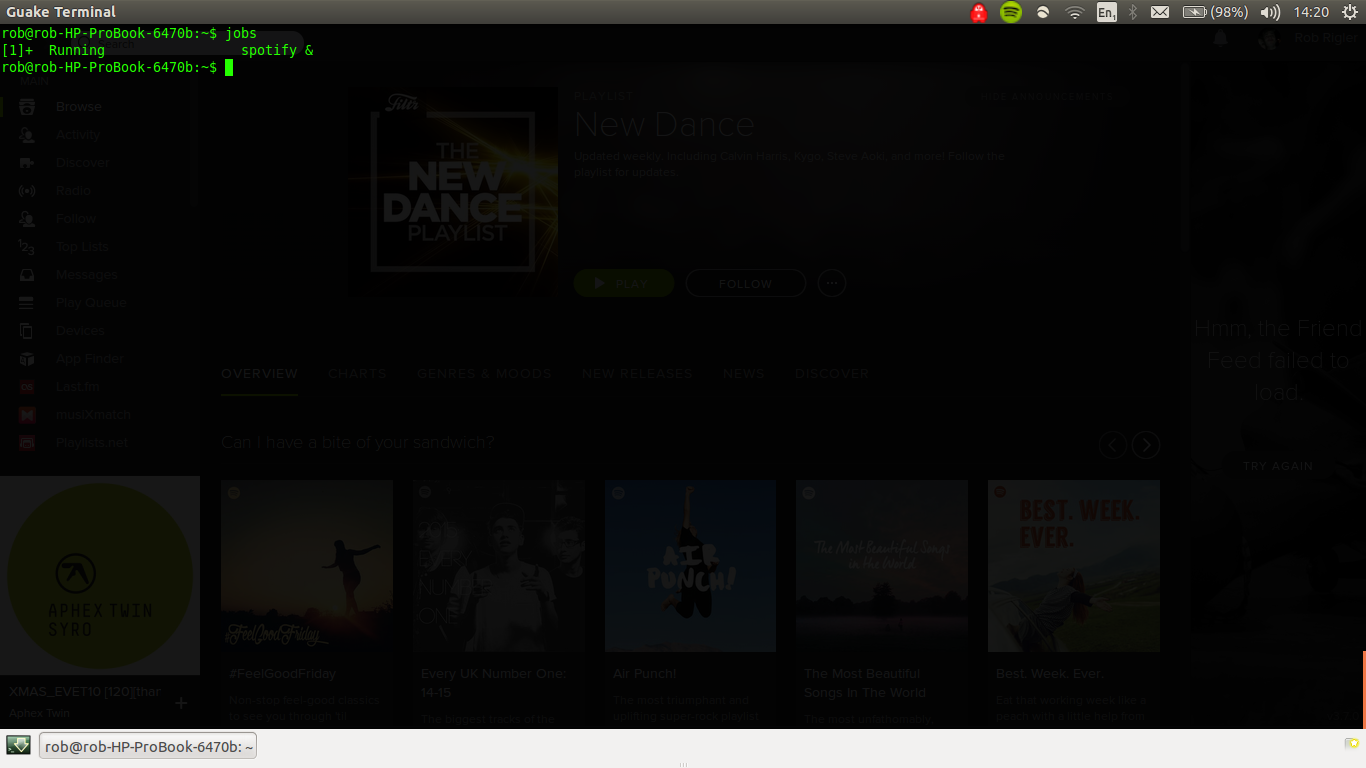
\includegraphics[scale =0.3]{Week14/nohup1.png} \\When I exit the shell, the 'spotify' application also closes.\\ \hfill
\pagebreak
Now, if I type 'nohup spotify \&' and look at the terminal jobs. It shows 'nohup spotify \& ' , but now if I type exit, the application will stay open regardless of the terminal.

\vspace{0.5cm} 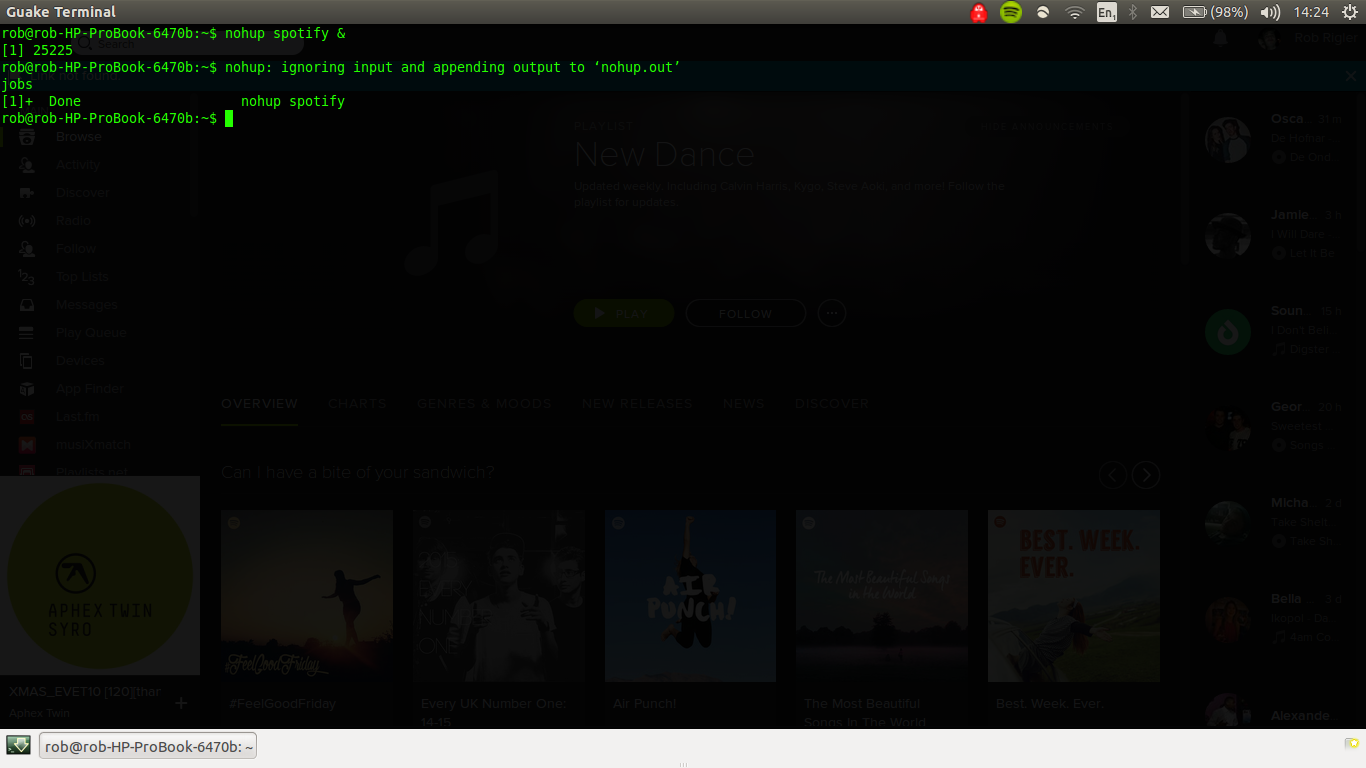
\includegraphics[scale =0.3]{Week14/nohup2.png}
\end{homeworkSection}
\end{homeworkProblem}
\pagebreak

\begin{homeworkProblem}[Week 17: Pipes and Sockets]
\begin{homeworkSection}{RPN Calculator}

This tasked asked me to modify the 'tcp-server' code to evaluate an expression in Reverse Polish Notation (RPN) and return the value to the client. Below I have included the modified code of 'tcp-server', and a screen-shot of the program working. The program is able to evaluate complex expressions such as:\\ \\ ' \textit{100 3 5 6 + * -} ' \\

which in prefix notation is : \\  

 '\textit{100 - 3 * (5+6) } ' \\ 

both of these expressions evaluate to 67.

\Cscript{Week17/code}{'tcp-server.cc' code}

Firstly to be able to evaluate an RPN expression, I needed to implement stack functionality. Lines 16 to 32 show me creating a stack. \\ I created an integer array to hold the values, and an integer to 'point' to the front on the stack. I then created the two funtions which would allow me to push and pop values to and from the stack respectively.\\

On lines 143 to 195 Is where I evaluated the RPN Expression.

Below is a screen-shot of the out on 'tcp-client'. It shows three separate expressions being evaluated : 
\begin{enumerate}
\item 100 3 5 6 + * - \hspace{1.2cm} (100 - 3 * (5+6))\\
\item 1000 345 - \hspace{2cm}  (1000 - 345)\\
\item 280 2 / 4 * \hspace{1.9cm} (4 * (280/2))
\end{enumerate}

\vspace{1cm}
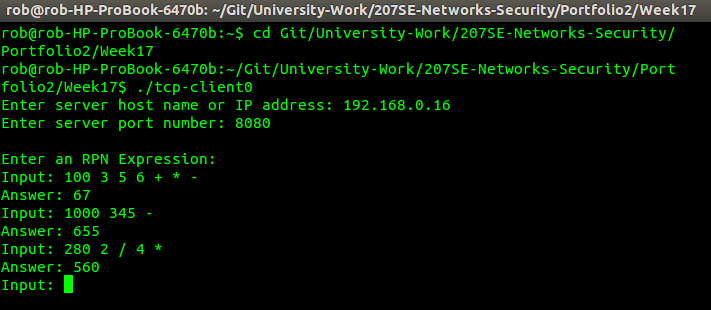
\includegraphics[scale=0.6]{Week17/rpn.png}



\end{homeworkSection}
\end{homeworkProblem}
\pagebreak
\begin{homeworkProblem}[Week 19: Security and Networks]	
	\begin{homeworkSection}{Activity 1: Access Control}
		\subsubsection{Domain Matrix}
		
		\vspace{1cm}
		
		\begin{tabular}{|l|c|c|c|c|c|c|c|c|} \hline
			& File1 & File2 & File3 & File4 & File5 & Printer & Screen1 & Mouse\\ \hline
			D1 & R & RW &   &     &    &    &   &   \\ \hline
			D2 &   &    & R & RWX & RW & W  &   &\\ \hline
			D3 &   &    & W  &     &    & W & W & R \\ \hline
		\end{tabular}
		
		
		\subsubsection{Access-List}
		\includegraphics[scale = 0.5, width = 18cm]{Week19/Access-list.png}
		\subsubsection{Compatibility-Lists}
		\includegraphics[scale = 0.5, width = 18cm]{Week19/Capabilitylist.png}		
		
		
	\end{homeworkSection}
	\pagebreak
	\begin{homeworkSection}{Activity 2: Hash Funciton}
		
		\Cscript{Week19/Hcode}{A Simple Hash function in C\#}
		
		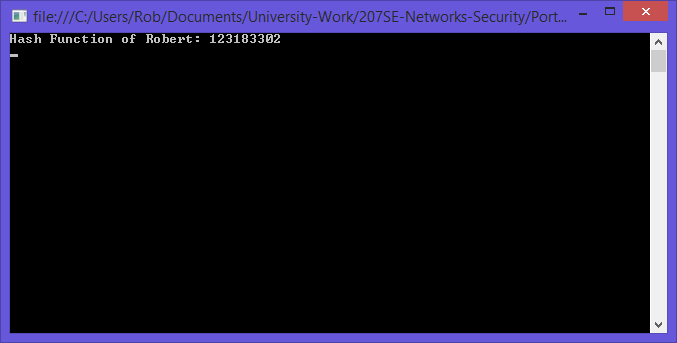
\includegraphics[scale = 0.7]{Week19/Hash}
	
	\end{homeworkSection}
	
\end{homeworkProblem}






\end{document}